\documentclass[]{scrartcl}
\usepackage{url}
\usepackage{xcolor}
\usepackage{graphicx}
\usepackage{listings}
\graphicspath{ {./img/} }
\usepackage{mathptmx}
\title{SentinelSuite}
\subtitle{IoT Project for Server Room Surveillance}
\author{Castorini Francesco}

\date{}

\begin{document}

\maketitle
\noindent
GitHub Repository: (\textcolor{blue}{\url{https://github.com/Il-castor/SentinelSuite}})
\newline
\newline
\noindent
This project presents a comprehensive exploration and implementation of an Internet of
Things (IoT) system designed to manage access control and environmental conditions
within a critical server room environment. The project incorporates the utilization of
ESP32 and ESP8266 microcontrollers for access and environmental policy enforcement,
respectively, alongside a Raspberry Pi serving as a central hub for data processing and visualization.

\section{Hardware}
For the realization of this project I used 3 different board:
\begin{enumerate}
	\item ESP32
	\item ESP8266
	\item Raspberry Pi
\end{enumerate}
The boards have the following hardware specs:
\newline 
\begin{center}

\begin{tabular}{|c|c|c|c|c|}
	\hline
	Board & Platform & CPU & RAM & Flash \\
	\hline
	ESP32 Dev & Espressif 32 & ESP32 & 240MHz & 4MB \\
	ESP8266 & Espressif 8266 & ESP8266 & 80MHz & 4MB \\
	Raspberry Pi 3B & - & 1.2GHz & 1GB & 32GB \\
	\hline
\end{tabular}
\end{center}
\noindent
All of these board have WiFi capability and expandibility for connecting external device.
\section{Access and Environmental Control}
\subsection{Access Policy}
The purpose of this policy is to ensure secure and controlled access to the server room by allowing only authorized staff to enter using a RFID badges and implementing measures to monitor and record access. This policy is implemented on a ESP8266.
\subsection{Environmental Policy}
The environmental monitoring policy for the server room is designed to ensure the safety and integrity of critical systems through constant and timely control of crucial environmental variables. This includes active monitoring of temperature, humidity, fire detection, and flood prevention. In the event of deviations from acceptable parameters, the system triggers immediate notifications to user and takes countermeasures. 
This policy is implemented on a ESP32.
\section{Software components}
I use \textbf{MQTT} because it is light, efficient and ideal for transmitting data in constrained
environments. In the future it will be possible to extend the sensor network.
\newline \newline
\textbf{Mosquitto} (\textcolor{blue}{\url{https://mosquitto.org/}}) is an open source message broker that implements
the MQTT protocol.
\newline \newline
\textbf{Node-RED} (\textcolor{blue}{\url{https://nodered.org/}}) is a programming tool for wiring together hardware
devices, APIs and online services. It is configured to process data and monitoring metrics coming from the boards.
\newline \newline
All these software are installed on Raspberry Pi which acts as a central hub.
\newline \newline
The complete project architecture is the following:
\begin{figure}[h!]
	\centering
	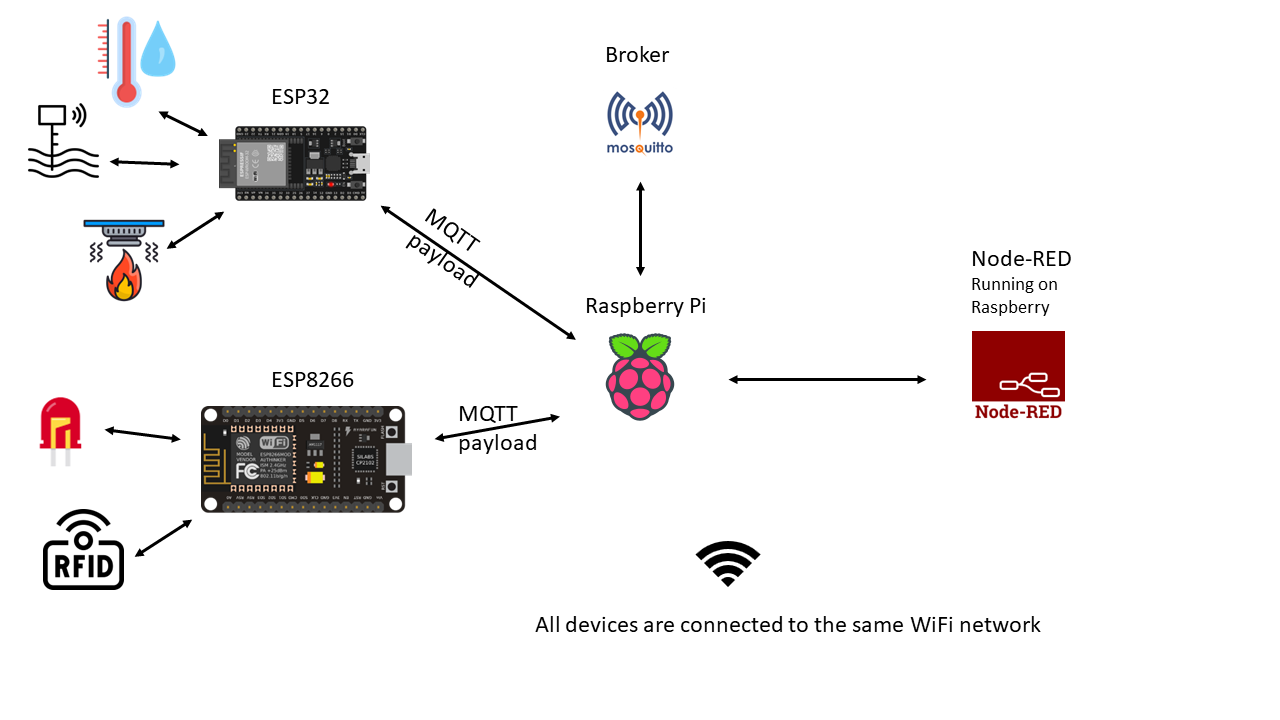
\includegraphics[width=\textwidth]{schema-iot.png}
	\caption{project architecture}
\end{figure}
\newpage
\noindent
I use \textbf{WiFi} because offers higher data transfer rates,  ensuring the efficient transmission of sensor data. Moreover, the infrastructure within a server room typically supports WiFi, reducing additional setup requirements. In the end, WiFi accommodates multiple simultaneous connections without substantial signal degradation, enabling both ESP devices to communicate concurrently with the Raspberry Pi.
\newline
Therefore, WiFi's balance of speed, reliability, and compatibility with the existing infrastructure makes it the preferred choice for facilitating seamless and robust communication between the ESP sensors and the central Raspberry Pi hub.
\section{Implementation}
For better management and use, both the esp8266 and the esp32 are dynamically configured. 
Once connected to the MQTT broker, the two boards subscribe to a pre-configured topic. The esp8266 is subscribed to: \textit{esp8266/configurazione}, while the esp32 is subscribed to \textit{esp32/configurazione}.

\subsection{ESP8266 and access policy}
Once subscribed to the topic, esp8266 receives the following JSON file:
\begin{figure}[h!]
	\centering
	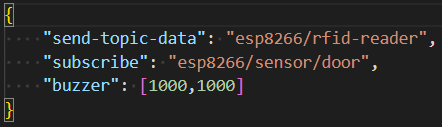
\includegraphics[width=\textwidth]{esp8266-config.png}
	\caption{ESP8266 JSON file}
\end{figure}
\newpage \noindent
A RFID reader is used to implement the access policy, and when a badge is near the reader, the contents of the badge are sent to the following topic: \textit{esp8266/rfid-reader}. Node-RED, once it receives the data, sends the string "1" on the topic \textit{esp8266/sensor/door} if the badge is registered, otherwise "0". If the board receives on the previous topic "1" then it turns on the green LED for 5 seconds and a sound is played by a buzzer; the frequency and duration of this sound can be set with the array specified in the last line of the JSON file. This means that it is possible to enter the server room. If it receives 0 it turns the led red for 5 seconds and this means that it is not possible to enter. After 5 wrong attempts the RFID reader is disabled and the led stays on red. Only from the dashboard of Node-RED the RFID reader can be unlocked. Through Node-RED it is possible to change this value. Each access attempt is recorded on a log that contains the badge ID and time of access.
\newline \newline \noindent
A video streaming is implemented on the raspberry that records real-time access to the server room to increase security.

\subsection{ESP32 and environmental policy}
This board implements environmental policies and once subscribed to the topic, it receives the following JSON file:
\begin{figure}[h]
	\centering
	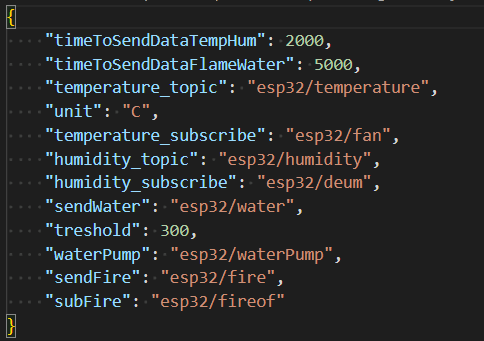
\includegraphics[width=\textwidth]{esp32-config.png}
	\caption{ESP32 JSON file}
\end{figure}
\newpage \noindent
The board, via the DHT11 sensor, monitors the temperature and humidity of the room, and if it has changed since the last measurement, then sends the new temperature and humidity on the following topics, respectively: \textit{esp32/temperature} and \textit{esp32/humidity}. Node-RED sends on the topic \textit{esp32/fan} the following values according to the range in which the temperature is:

\begin{itemize}
	\item less than 20° the string "0" is sent and the fan is not turned on
	\item between 20° and 30° the string "1" is sent and the fan is turned on at minimum 
	\item between 30° and 35° string "2" is sent and the fan is turned on at an average value
	\item greater than 35° string "3" is sent and the fan is turned on at maximum
\end{itemize}
These thresholds can be changed from Node-RED. In addition, it is possible to send the temperature in either Celsius or Fahrenheit by setting the F or C value in "units" in configuration file.
\newline
An RGB led is used to simulate the fan turning on where the fan states are mapped in the following colors: white, purple, green, red.
\newline\newline
On the topic \textit{esp32/deum} string "0" is sent if the humidity is less than 40\%, it can be changed via Node-RED dashboard, otherwise if it is higher string "1" is sent and the dehumidifier is turned on. It is simulated with the following colors on the RGB led: black, meaning the led is off and orange.
\newline \newline
Through a water level sensor the water level is measured and if the threshold specified in "treshold" is exceeded then the string "on" is sent on topic \textit{esp32/water} otherwise the string "off" is sent. Node-RED, based on the value it receives, turns a water pump on or off by sending the string "1" or "0" on the topic \textit{esp32/waterPump}. The pump is simulated by turning on a blue SMD LED, or pink if the water pump is not running.
\newline \newline
Finally, through a fire sensor, the presence of flames is detected. If they are detected, string "1" on topic \textit{esp32/sendFire} is sent to Node-RED which sends string "1" on topic \textit{esp32/fireof} to turn on the fire system. It is simulated by flashing the red SMD LED 3 times. If no flames are detected then string "0" is sent and the SMD led lights pink.

\subsection{Node-RED dashboard}
The main purpose of this dashboard, created with Node-RED, is to provide a real-time visualization of the data sent by the two ESP.
\newpage
\begin{figure}[h]
	\centering
	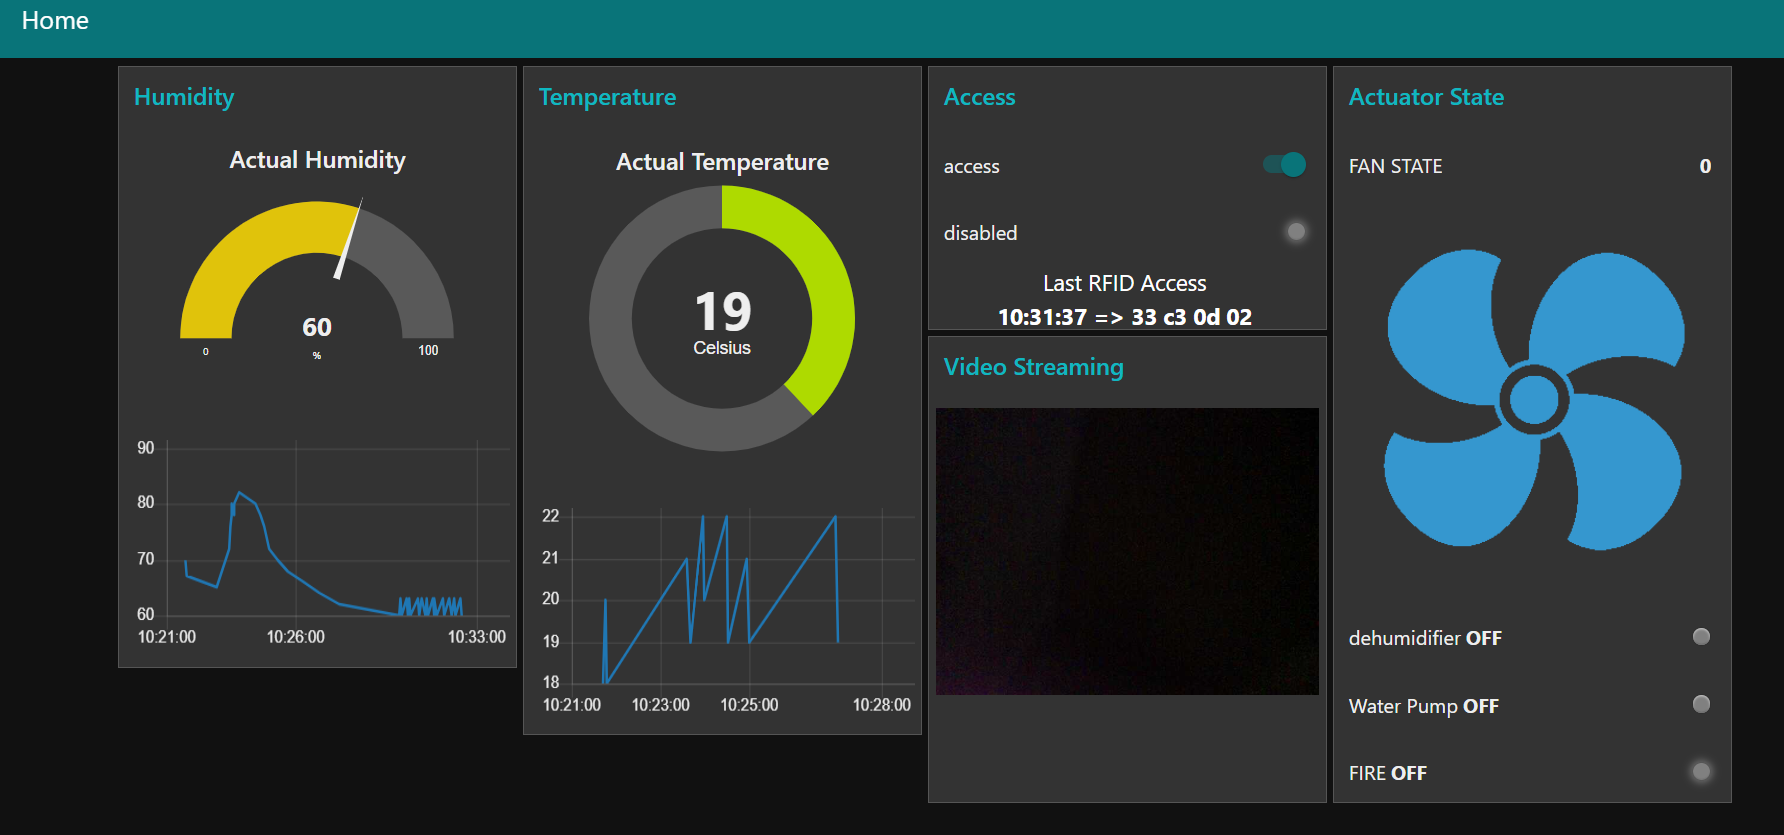
\includegraphics[width=\textwidth]{node.red-dashboard.png}
	\caption{Node-RED dashboard}
\end{figure}
\noindent
Its structure is divided into several key sections to provide a comprehensive overview of the environmental, access and control conditions of the actuators in the server room.
\newline\newline
The first section, on the left, is devoted to displaying humidity and temperature through two separate graphs for each. These graphs provide both a real-time and historical representation of changes in temperature and humidity.
\newline\newline
Important is the access control section that provides a streaming video of the monitored environment along with the last access made. In addition, it is possible to disable access if necessary.
\newline\newline
Finally, the dashboard includes a section dedicated to the status of connected actuators, allowing the user to view the real-time status of these devices such as the air conditioning system.
\end{document}
